\documentclass[a4paper,ngerman, 11pt]{report}

%% Päambel
\usepackage[T1]{fontenc}
\usepackage[utf8]{inputenc}
\usepackage{babel}
\usepackage{cite}
\usepackage{xcolor}
\newcommand\Diskussionspunkt[1]{\textcolor{red}{#1}}

\usepackage{url}
\usepackage{hyperref}

% Grafikpaket laden
\usepackage{graphicx}

% Quelltext
\usepackage{listings}
 \usepackage{color}
 
 \definecolor{middlegray}{rgb}{0.5,0.5,0.5}
 \definecolor{lightgray}{rgb}{0.8,0.8,0.8}
 \definecolor{orange}{rgb}{0.8,0.3,0.3}
 \definecolor{yac}{rgb}{0.6,0.6,0.1}
 
  \lstset{
   basicstyle=\scriptsize\ttfamily,
   keywordstyle=\bfseries\ttfamily\color{orange},
   stringstyle=\color{green}\ttfamily,
   commentstyle=\color{middlegray}\ttfamily,
   emph={square}, 
   emphstyle=\color{blue}\texttt,
   emph={[2]root,base},
   emphstyle={[2]\color{yac}\texttt},
   showstringspaces=false,
   flexiblecolumns=false,
   tabsize=2,
   numbers=left,
   numberstyle=\tiny,
   numberblanklines=false,
   stepnumber=1,
   numbersep=10pt,
   xleftmargin=15pt
 }


%%  Variablen
\newcommand{\authorName}{Ladina Bilgery \and Thomas Wieling}
\newcommand{\auftraggeber}{Interessengemeinschaft Wetterstation Arbon}
\newcommand{\auftragnehmer}{Interstaatliche Hochschule für Technik NTB}
\newcommand{\projektName}{User Interface und Datenmanagement für die Wetterstation Arbon}
\title{\projektName~(Fachmodul)}
\author{\authorName}
\date{\today}

%%  Create a shorter version for tables. DO NOT CHANGE 
\newcommand\addrow[2]{#1 &#2\\ }
\newcommand\addheading[2]{#1 &#2\\ \hline}
\newcommand\tabularhead{\begin{tabular}{lp{13cm}}
\hline
}
\newcommand\addmulrow[2]{ \begin{minipage}[t][][t]{2.5cm}#1\end{minipage}
   &\begin{minipage}[t][][t]{8cm}
    \begin{enumerate} #2   \end{enumerate}
    \end{minipage}\\ }
\newenvironment{usecase}{\tabularhead}
{\hline\end{tabular}}



%%  Beginn Dokument
\begin{document}
\pagenumbering{roman}
\begin{titlepage}
\maketitle
\thispagestyle{empty} 

\begin{verbatim}

\end{verbatim}


  \begin{tabular}[t]{ll}
	Projekt:       & \quad \projektName \\[1.2ex]
	Auftraggeber:  & \quad \auftraggeber\\[1.2ex]
	Auftragnehmer: & \quad \auftragnehmer\\[1.2ex]
  \end{tabular}

\begin{tabular}{|p{3 cm}|p{3 cm}|p{5 cm}|}
\hline
\textbf{Version} & \textbf{Datum} & \textbf{Autor(en)} \\
\hline
\hline
1.0 & 16.11.2017 & \authorName \\
\hline
\end{tabular}
\end{titlepage}

\setcounter{page}{2}
\tableofcontents          
\clearpage
\pagenumbering{arabic}


%%%%%%%%%%%%%%%%%%%%%%%%%%%%%%%%%%%
%%  Einführung
%%%%%%%%%%%%%%%%%%%%%%%%%%%%%%%%%%%
\chapter{Einführung}
Ziel des Fachmoduls, Aufträge, Vorgehensweise, Vorstellung Wetterstation Arbon

\Diskussionspunkt{Foto Wetterstation}


\Diskussionspunkt{Beispiel für eine Bildintegration inkl. Referenz darauf:}
\begin{figure}[htbp]
	\centering
	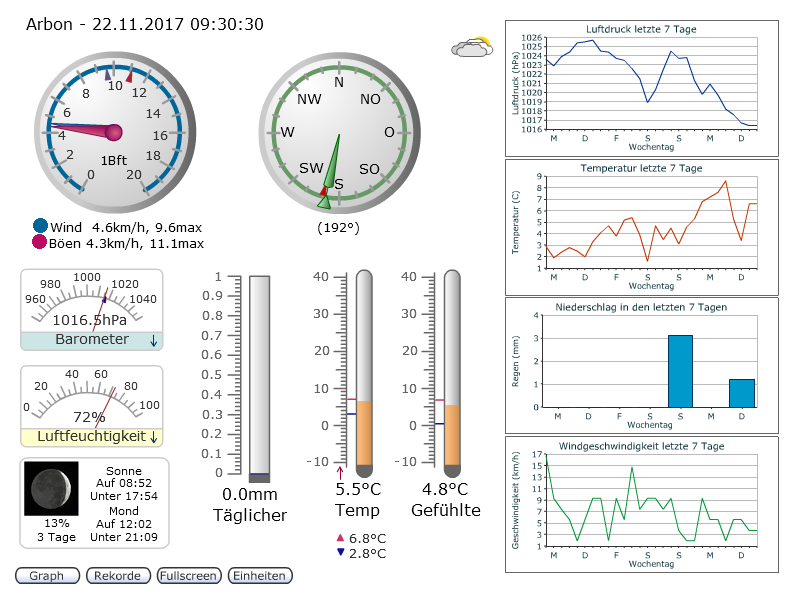
\includegraphics[width=0.9\linewidth]{img/grafik}
	\caption{eine Grafik ohne Sinn und Verstand}
	\label{img:grafik-dummy}
\end{figure}

Weiterhin wollen wir an dieser Stelle Bezug auf die Grafik
\ref{img:grafik-dummy} auf Seite \pageref{img:grafik-dummy} nehmen, was uns
hiermit gelungen sein dürfte. Latex passt die Seitenzahl aber auch die Nummer
der Grafik automatisch an, wir müssen uns um nichts kümmern.

%%%%%%%%%%%%%%%%%%%%%%%%%%%%%%%%%%%
%%  Hauptteil
%%%%%%%%%%%%%%%%%%%%%%%%%%%%%%%%%%%
\chapter{Hauptteil}

\section{IST-Zustand}
\Diskussionspunkt{Hardware und Software, 
Skizze, 
Übersicht, 
Verbindungen/Verknüpfungen untereinander}
\Diskussionspunkt{Bild}

\subsection{Installierte Komponenten}

Die Wetterstation Arbon besteht aus folgenden Sensoren bzw. Sensor-Einheiten:
\begin{itemize}  
\item Webcam
\item Kombi-Wetter-Transmitter
\item Wassertemperatur-Sensor
\item Pegel-Sensor (defekt)
\end{itemize}


Die Webcam ist 360 Grad drehbar, schwenkbar, verfügt über eine Zoomfunktion und kann ferngesteuert werden.  Der Kombi-Wetter-Transmitter vereint mehrere Sensoren in einem Gehäuse. Dies sind Windgeschwindigkeit und -richtung, Lufttemperatur, relative und absolute Luftfeuchtigkeit, Regenmenge und Luftdruck. Der Wassertemperatur-Sensor besteht aus mehreren PT100-Widerständen, die in einem Kunststoffrohr im Abstand von 20cm montiert sind. Bei den Temperaturwiderständen ist einer defekt. Der Wert dieses Sensors wird mit Hilfe der beiden Nachbar-Wiederständen interpoliert. Den defekten Temperaturwiderstand zu ersetzen ist zu aufwändig. Der Pegelsensor ist im gleichen Kunststoffrohr verbaut wie die Temperatur-Widerstände und misst den hydrostatischen Druck. Das Kunststoffrohr ist gegen den Seegrund hin offen und nach oben verschlossen.

Die Wetterstation ist auf einem Pfahl ausserhalb des Hafens Arbon montiert. Auf dem Pfahl befindet sich ein kleiner Schaltschrank, jedoch keine Auswertelogik. Sämtliche Daten werden in IP-Pakete verpackt und über eine Glasfaser-Leitung an den Server gesendet.

Die verbauten Komponenten sind in der Grafik \ref{img:HW-Aufbau} schematisch dargestellt.

\begin{figure}[htbp]
	\centering
	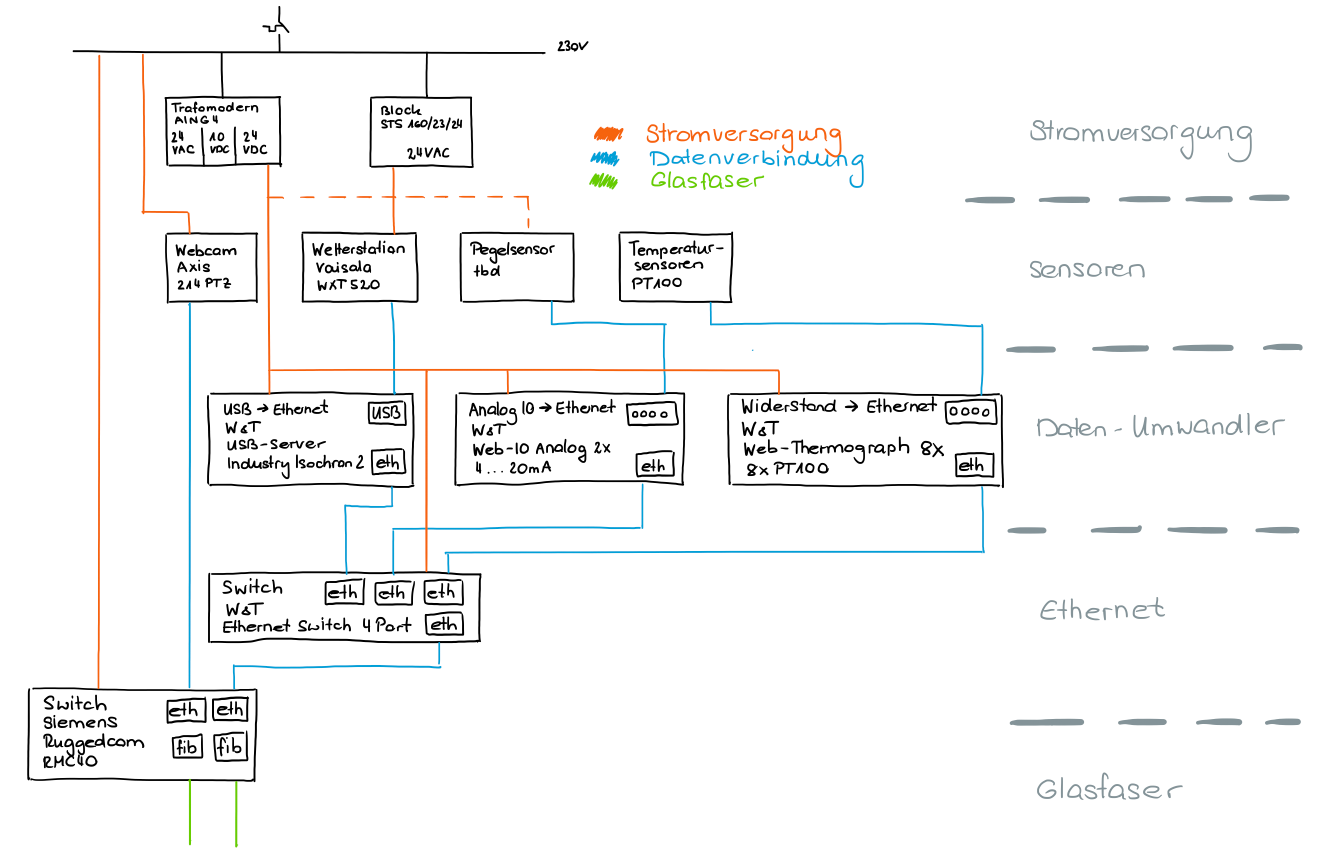
\includegraphics[width=1\linewidth]{img/HW-Aufbau}
	\caption{Hardware-Aufbau der Wetterstation Arbon}
	\label{img:HW-Aufbau}
\end{figure}

  
\subsection{Was ist Openfile64Light?}
Openfile64Light ist ein CMS der Firma Screenbox. Mit diesem ist es möglich um mit ein paar Klicks eine Webseite erstellt werden kann. Es kann direkt in einem Browser der gewollte Text sowie Bilder und Graphiken eingesetzt werden. Des Weiteren können auch Formulare, Menüs und Applikationen einfach mit einem Mausklick eingesetzt werden. Der Nachteil des CMS ist, dass auf die Seite selber keine eigenen HTML, CSS oder Javascript Dateien erlaubt. Somit können eigene Änderungen an der Webseite nicht durchgeführt werden und ist man vom CMS abhängig. Eigene Änderungen oder dynamische Inhalte, werden in openfile64Light als sogenannte Applikationen behandelt. Worin unterscheidet sich openfile64Light zu openfile64? Die Light Version des CMS lässt folgende Funktionen nicht zu:
\begin{itemize}
\item Mehrsprachig (D/E/F)
\item Automatische Volltextsuche und Sitemaperstellung
\item Rollen- und gruppenbasierende Benutzerverwaltung
\end{itemize}


\subsection{Wie und wo werden Applikationen erstellt?}
Eine Möglichkeit um eigene Änderungen zu tätigen ist, eine sogenannte Applikationen zu erstellen. Die gewünschte Applikation, d.h. eine PHP Referenzdatei, welche auf die HTML, Javascript und CSS Dateien in einem eigenen Ordner verweisen, müssen im Ordner application werden und in der Datenbank in der Tabelle applications gespeichert werden. Um eigene Applikationen in das CMS einzubinden, muss dies über Screenbox gehen. Diese erstellen dort die Applikation in der Datenbank und vergeben auch die Namen, damit diese auf der Webseite ausgewählt werden kann. Die geschieht gegen einen Unkosten Beitrag von 75 Schweizer Franken.

\subsection{Wetterapplikation Wassersport und Touristik}
Die Wetterdaten der Wetterstation Arbon werden von Weather-Display ausgewertet und von Weather-Display Live dargestellt. Die Applikation Weather-Display Live wurde im Auftrag der IG Wetterstation Arbon erstellt und auf Deutsch übersetzt. Bei der Übersetzung hat es Fehler gegeben, des Weiteren läuft die Applikation nur mit Flash, welches nicht von allen Geräten unterstützt wird. Um dieses Problem aus der Welt zu schaffen, macht die Seite einen Screenshot der aktuellen Daten beim Aufrufen der Seite. Mit dem Screenshot gibt es aber keine dynamische Seite, d.h. die Anzeigen ändern beispielsweise bei einer Richtungsänderung des Windes die Richtung nicht mit.  
\begin{figure}[htbp]
	\centering
	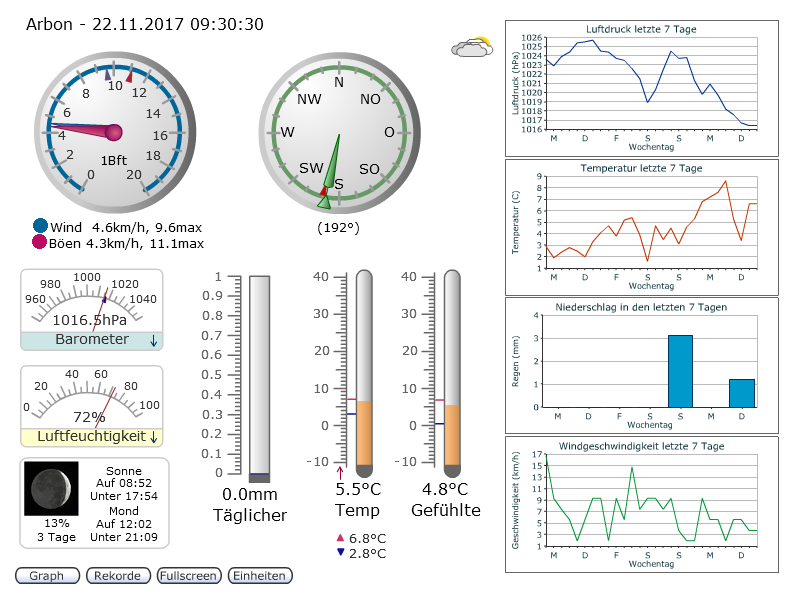
\includegraphics[width=0.9\linewidth]{img/grafik}
	\caption{Datenanzeige wetter-arbon.ch}
	\label{img:grafik-dummy}
\end{figure}

\subsection{Warum wird kein Flash mehr gebraucht?}
Zu beginn des Internetzeitalters, war Flash essentiell für dynamische Webseiten. Mit ihm konnten einfach dynamische Inhalte erstellt und administriert werden. Jedoch gab es immer wieder gravierende Sicherheitslücken und Weiterentwicklungen im Bereich Web. Mit dem aufkommen der Smartphones wurde Flash immer weiter verdrängt durch HTML5 und Javascript. Nicht zuletzt auch durch ein Kommuniqué von Steve Jobs. In diesem erklärt er warum seine Firma (Apple) nicht auf Flash, sondern HTML5 und Javascript setzt. Einer der Gründe für dieser Entscheidung ist, dass Flash keine open-source Software ist. D.h Adobe kontrolliert das System. Hierbei erwähnt Steve Jobs auch das Apple ein closed-source system ist, sie jedoch an einen offenen Webstandard glauben. Der zweite Grund ist warum Apple sich nicht für Flash entschieden hat ist, dass die Videos bzw. Games seit diesem offenen Brief aus dem Jahr 2009 auch in den neuen Standards, H.264, erhältlich ist. Der dritte Grund, das Apple nicht auf Flash gesetzt hat ist die Sicherheit. Aus Untersuchungen im Jahr 2009 ging hervor, dass die ihre Macs abstürzen. Dies kommt durch die Flashsoftware von Adobe. Dazu kommt, dass Flash auf den mobilen Geräten von Apple nicht sicher lief. Mehrmals wurde Adobe gefragt um eine laufende Version zu erstellen, dies hat Adobe jedoch nicht geschafft. Aus diesen Gründen hat Apple, welcher einer der Vorreiter von Smartphones war, sich entschieden um Flash nicht zu benutzen. Dadurch haben auch andere Hersteller von mobilen Geräten nachgezogen und auf Flash möglichst verzichtet. \cite{Apple:ThoughtsOnFlash} \\
Der wichtigste Grund ist das Adobe ab 2020 Flash nicht mehr weiterentwickelt und keine Updates mehr herausgeben wird. Dies aufgrund der oben genannten Tatsachen und das zur heutigen Zeit vielmals Flash umgangen wird und andere Lösungen gebraucht werden. Aufgrund von dies wird ab 2020 auch kein Browser mehr das Plugin zulassen und Seiten welche Flashinhalte benutzen sind nicht mehr Vollständig verfügbar. Somit ist auch die Wetter-Arbon Seite von dieser Tatsache betroffen. Um trotzdem erreichbar zu sein auf Endgeräte ohne Flash wird in der Wassersport.php bzw. Touristik.php Datei der Entscheid gefällt ob die Flash-Seite oder die Bild-Seite geöffnet wird, im Code des Wassersport.php-File oder im Touristik.php-File, je nachdem welche Seite geöffnet wird gefällt. Zuerst wird abgefragt ob das object eine Flashplayerversion hat, so ja wird die index.html Seite geöffnet. Ist die if abfrage negativ wird die WDL.png geöffnet. \cite{Adobe:FlashTheFutureofInteractiveContent}

\begin{lstlisting}
if (swfobject.hasFlashPlayerVersion("1")) {
document.write('
<iframe 
src="https://www.wetter-arbon.ch/WDL/index.html">
</iframe>');
} 
else {
document.write('
<img class="pageImage" 
src="https://www.wetter-arbon.ch/WDL/WDL.png" alt="Bodensee West" 
/>');
}
\end{lstlisting}

\subsection{Mobile Webseite}
Zusätzlich zur Desktop-Seite, auf welcher alle Informationen verfügbar sind, gibt es eine mobile abgespecktere Version der Wetterstation, siehe \ref{img:mobilewebseite} auf Seite \pageref{img:mobilewebseite}, diese ist erreichbar unter m.wetter-arbon.ch. Auf dieser werden die zwei aktuellsten Bilder der Touristikseite, bzw. der Wassersportseite auf einer Seite dargestellt. Zusätzlich gibt es einen Link welche die Bilder der Webcam, sowie deren Steuerungseinheit darstellt.
\begin{figure}[htbp]
	\centering
	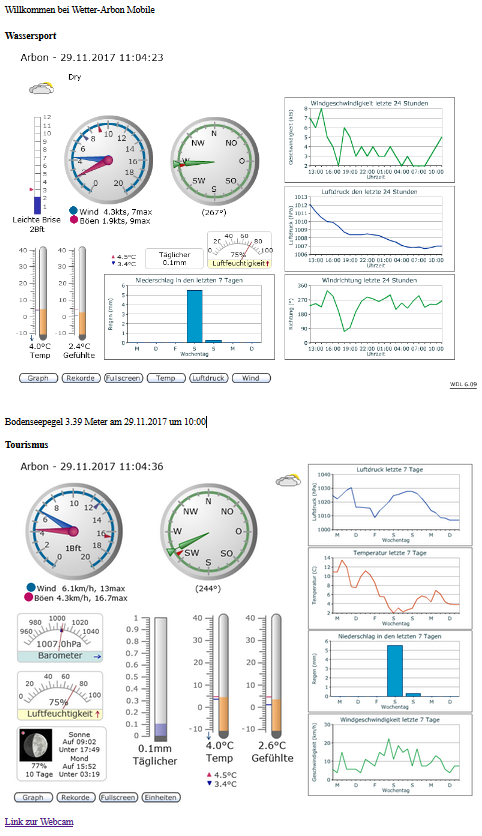
\includegraphics[width=0.9\linewidth]{img/mobile_webseite}
	\caption{Datenanzeige m.wetter-arbon.ch}
	\label{img:mobilewebseite}
\end{figure}


\subsection{Sturmwarnung}
Die Seite mir der Sturmwarnung, siehe \ref{img:sturmwarnung} auf Seite \pageref{img:sturmwarnung}   gibt es im eigentlichen nicht mehr. Es wird nur noch ein Link zur Verfügung gestellt um auf die kantonale Sturmwarnseite zu kommen. Der Grund dafür ist das die verlinkte Seite, welche zuerst integriert war nicht dem HTTPS sondern dem HTTP Standard entspricht. Die Daten der Sturmwarnung werden mit dem deutschen Wetterdienst in Stuttgart sowie Meteo Schweiz erstellt. Zu beachten ist hierbei, dass die Sturmwarnungen Bürozeiten haben. D.h. konkret vom 1. April bis 31 Oktober zwischen 6 und 22 Uhr und vom 1. November bis 31. März zwischen 7 und 20 Uhr. 
\begin{figure}[htbp]
	\centering
	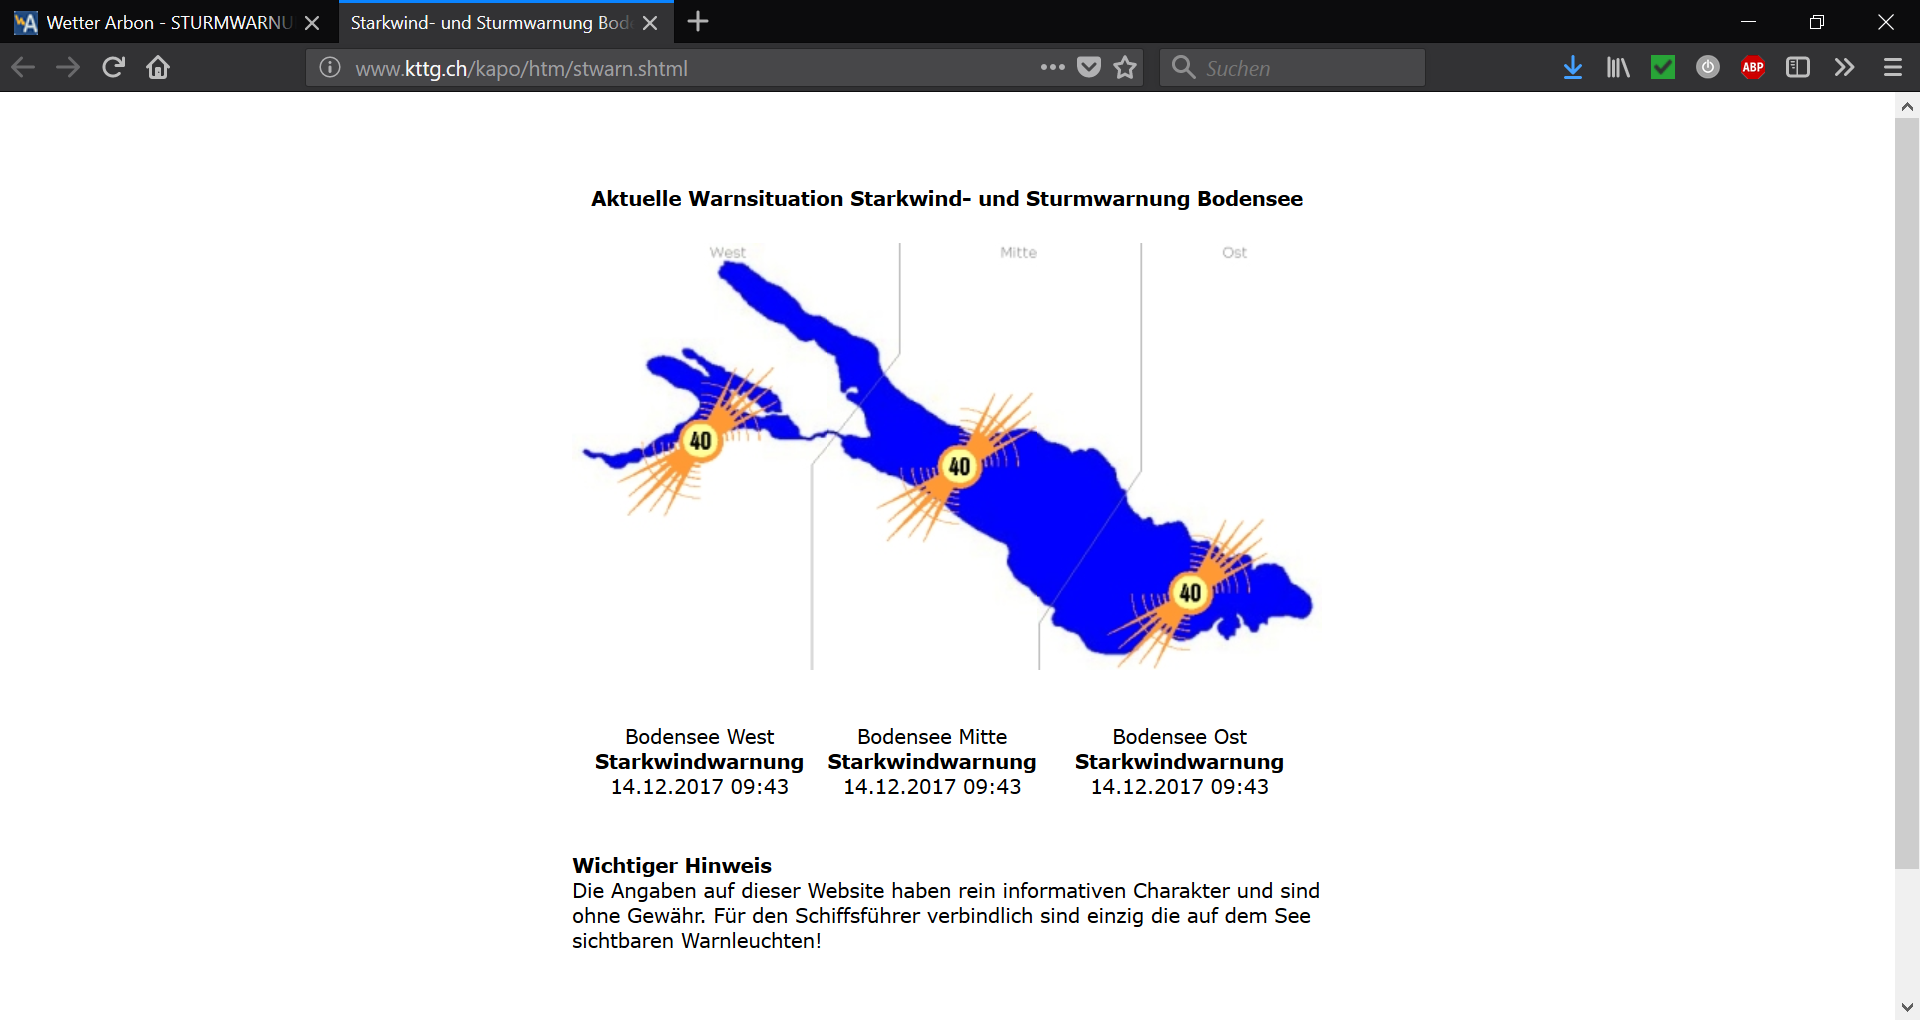
\includegraphics[width=0.9\linewidth]{img/sturmwarnung}
	\caption{Sturmwarnung vom Kanton Thurgau}
	\label{img:Sturmwarnung}
\end{figure}

\subsection{Welche Komponenten hat die Datenbank?}
Für die Webseite und die Wetterstation, hat es vier verschiedene Datenbanken. Diese werden in diesem Kapitel einzeln behandelt und erklärt wie Sie zusammenhängen bzw. welche Rolle sie für die Webseite spielen. Die vier Datenbanken heissen:
\begin{itemize}  
\item igwetter meteotmpl
\item igwetter wettertest
\item gwetter wp0
\item gwetter openfile64Light
\end{itemize}

Die Datenbank igwetter meteotmpl beinhaltet alle relevanten Datenpunkte, d.h. von der Temperatur bis zur Windrichtung. In dieser Datenbank sind jedoch keine Daten vorhanden und dient momentan nur als Template.\\
Die zweite Datenbank welche nicht aktiv ist, heisst igwetter wp0, diese wurde für eine kurze Zeit für eine Wordpress-Seite benutzt.\\
Die dritte Datenbank ist die igwetter wettertest. Diese ist im Gegensatz zu den vorherigen beiden Datenbanken im Gebrauch. In der Tabelle wx data sind die Daten ab dem 25.02.2015 bis zum jetzigen Zeitpunkt gespeichert. Daten zwischen dem 14.07.2012 und 25.02.2015 sind nicht in der Datenbank hinterlegt. Vor diesem Zeitpunkt bis zum 25.02.2005 sind die täglichen Minimum, sowie Maximum Daten in der Tabelle tblgestern gespeichert.\\
Anders als bei den vorherigen Datenbanken hat die igwetter opfile64Light Datenbank eine Funktion für die Webseite. In diesem Fall ist die ganze Webseite abhängig von dieser, denn das CMS basiert auf einer Datenbank. Dies wurde im Kapitel Wie und wo werden Applikationen erstellt bereits erläutert. Für die BA, sowie das Fachmodul ist nur die Tabelle applications interessant, denn dort werden die Applikationen unter einem bestimmten Namen abgespeichert und aufgerufen. Die Webseite weiss dann welche Datei sie öffnen muss, damit die Applikation läuft.\\


\subsection{Daten vom 14.7.2012 bis 25.02.2015}
Die Wetterstation in Arbon musste im Jahr 2012 vom Netz genommen werden, weil sich die technischen Probleme überhäuften. Nachdem sich immer mehr Interessenten meldeten, dass die Wetterstation wieder aufgebaut werden muss, hat man 2015 die Arbeiten wieder aufgenommen um diverse Modernisierungen vorzunehmen. Dies ist der Grund warum es zwischen 2012 und 2015 keine Daten der Wetterstation gibt. ~\cite{Felix:ErweiterteHorizonte}

\subsection{Wofür sind die .txt Files}
Die Weahter-Display Software speichert alle Daten welche von der Wetterstation kommen in ein .txt File. Das Weather-Display live nimmt die Daten anschliessend direkt aus diesem File um die Anzeigen zu erstellen. Die Daten werden in 4 verschiedenen Textfiles mit unterschiedlichen Funktionen gespeichert.
\begin{itemize}  
\item clientraw.txt
\item clientrawextra.txt
\item clientrawhour.txt
\item clientrawdaily.txt
\end{itemize}

Die clientraw.txt Datei enthält die aktuellen Wetterdaten der Station. Der Intervall der Aktualisierung dieser Datei wird in der Datei wdlconfig.xml eingestellt. Im Fall von Arbon wird die Datei alle 5 Sekunden aktualisiert.  Hier werden auch die restlichen Parameter bzw. Einheiten in der die Daten gespeichert werden sollen eingestellt. Die clientrawextra.txt enthält die historischen Extremwerte. Die Datei clientrawhour.txt enthält die aufgezeichneten Daten der letzten Stunde im Minutentakt.\cite{WeatherDisplay}


\subsection{Wie kommen die Daten in die Datenbank?}
Die Daten, welche von der Wetterstation an einen Server in der Uni Liechstein gesendet werden, werden über die Software Weather-Display direkt in die Datenbank ig wettertest Tabelle wxdata geschrieben. Die Daten werden hier im Minutentakt eingelesen.

\subsection{Webcam}
Zur Wetterstation Arbon gehört auch eine Webcam der Marke Axis. Diese ist auch wieder über ein Applikationsplugin in die Webseite integriert. Auf dieser können per schort links sechs verschiedene Positionen angefahren werden:
\begin{itemize}  
\item Home
\item See Nord
\item Schloss
\item Hafeneinfahrt
\item Horn
\item Seerettung
\end{itemize}
 In der Betriebseigenen Software lassen sich viele Parameter ändern bzw. Beschränken. Sowie die Vergrösserung. Diese ist jedoch aus  Datenschutzgründen die 4-fache Vergrösserung limitiert, möglich wäre eine 216-fache Vergrösserung. Neben den voreingestellten Positionen, kann die Kamera auch frei Positioniert werden. Dies freie Positionierung erfolgt über Pfeile, sowie die Plus und Minus am Bildrand, jenachdem welcher Button geklickt wird, sendet die Webseite das Kommando an die Webcam. Dies geschieht mittels Javascript, wie man dem folgenden Code entnehmen kann.
 
\begin{lstlisting}
 <div class="container webcam" id="webcam_585">
	<div class="up"></div>
	<div class="left"></div>
	<div class="right"></div>
	<img class="pageImage" src="https://webcam.wetter-arbon.ch/mjpg/video.mjpg" alt="" />
	<div class="down"></div>
	<div class="zoomOut"></div>
	<div class="zoomIn"></div>
	<span class="home">Home</span>
	<span class="SeeNord">See Nord</span>
	<span class="Schloss">Schloss</span>
	<span class="Hafeneinfahrt">Hafeneinfahrt</span>
	<span class="Horn">Horn</span>
	<span class="Seerettung">Seerettung</span>
</div>
<script type="text/javascript">
	function changeWebCam(command) {
		var urlAddition;
		
		switch (command) {
			case 'up':
			case 'down':
			case 'left':
			case 'right':
			case 'home':
				urlAddition = 'move=' + command;
				break;
				
			case 'zoomIn':
				urlAddition = 'rzoom=2500';
				break;
				
			case 'zoomOut':
				urlAddition = 'rzoom=-2500';
				break;
				
			case 'SeeNord':
			case 'Schloss':
			case 'Hafeneinfahrt':
			case 'Horn':
			case 'Seerettung':
				urlAddition = 'gotoserverpresetname=' + command;
				break;
				
		}
		
		console.log('changeWebCam');
		$.get('https://webcam.wetter-arbon.ch/axis-cgi/com/ptz.cgi?camera=1&' + urlAddition);
	}
\end{lstlisting}

\section{Problemanalyse}
\Diskussionspunkt{Beschreibung, 
Begründung, 
Erkenntnisse aus IST-Analyse}

\subsection{Hardware}
Sowohl die Webcam, als auch der Kombi-Wetter-Transmitter funktionieren einwandfrei. Der defekte Temperaturwiderstand wird akzeptiert, da dessen Wert interpoliert werden kann. Der Pegel-Sensor hingegen ist defekt und muss ersetzt werden. Der bisherige Sensor nutzte das Prinzip der hydrostatischen Druckmessung. Für die Pegelmessung konnten wir drei verschiedene Messprinzipien eruiert, die eingesetzt werden können:

\begin{itemize}  
\item Hydrostatische Druckmessung
\item Ultraschall-Distanzmessung
\item Radar-Distanzmessung
\item Time-of-light-Distanzmessung
\end{itemize}

\subsection{Webseite}
Die Webseite der IG Wetterstation Arbon, ist bei auf den Seiten Wetter Touristik bzw. Wassersport auf einem alten Stand der Technik. Es wird Flash benutzt, welcher heutzutage schon fast verpönt ist. Das Problem hierbei ist, dass viele Geräte Flash nicht mehr unterstützen und die Lösung mit dem Screenshot der aktuellen Verhältnisse auch keine optimale Lösung ist. Weiter fällt bei der Begutachtung der Webseite das es einige Schreibfehler bzw. Übersetzungsfehler gibt, welche die Webseite auch nicht in einem besseren Licht da stehen lässt. Weiter ist die Wetterapplikation nicht nach dem Prinzip responsive Design aufgebaut, welches in der heutigen Zeit ein wichtiger Bestandteil einer Webseite ist. Nebst diesen erwähnten Problemen ist es auch nicht mehr möglich um auf der Webseite selber Sturmwarnungen anzuzeigen. Das Problem hierbei ist das die Webseite auf welche verlinkt wurde mit dem HTTP standard erstellt wurde und nicht mit HTTPS.

\subsection{Datenbank}
Werden die Datenbanken zum jetzigen Zeitpunkt angeschaut, scheint es chaotisch zu sein. Im Grunde werden nur die igwetter openfile64Light und die igwetter wettertest Datenbank benutzt. Das Problem hierbei ist das auf dem ersten Blick nicht sichtbar ist, was wo gemacht wird und welche Datenbank für wofür zuständig ist. Des weiteren wird nicht nur eine Datenbank sondern auch .txt Files benutzt um ein Backup zu erstellen, sowie die aktuellen Daten zu speichern. Die historischen Daten in der Datenbank sind nicht vollständig, zum einen gibt es für den gesagten Zeitraum zwischen 2012 und 2015 keine Daten und zum anderen werden die seit dem erstellten Daten nicht auch in die "historische" Datenbank abgelegt.

\subsection{Webcam}
Die Limitierung des Zooms der Webcam sollte möglichst dynamisch sein. Im jetzigen Zustand ist es nur möglich überall den gleichen Zoomfaktor zu benutzen, obwohl dies nicht notwendig wäre. Beispielsweise könnte der Zoomfaktor auf den See hinaus um einiges grösser sein als auf die umliegenden Häuser. Das Problem hierbei ist jedoch, dass sich dies nicht in der angebotenen Software der Webcam umsetzen lässt und somit andere Möglichkeiten evaluiert werden müssen.

\subsection{SMS Alarmierung}

\section{SOLL-Zustand}
\Diskussionspunkt{Lösungsansätze = zu entwickelnde Artefakte, 
Resultat aus Literaturrecherche, 
Konzepte}

\subsection{Webseite}
Die Webseite soll auf dem neusten Stand der Technik gebracht werden. Konkret heisst dies, der Flash wird ausgemustert und die Applikation wird auf HTML5 und Javascript umgestellt. Die Webseite soll zudem im responsive Design entwickelt werden, damit auch auf mobilen Geräten die aktuelle Wetterlage sichtbar ist. Die dynamischen, sowie auch die teilweise statischen Anzeigen, werden wo möglich mithilfe der Javascript Bibliothek D3.js erstellt, hiermit lassen sich ansehnliche und moderne Grafiken erstellen. Die Grafiken, sollten so gestaltet sein das auch Sehbehinderte Personen erkennen wie das Wetter momentan ist. Das heisst beispielsweise, dass die Farben auch für Farbenblinde unterscheidbar sein sollten oder blinde Personen anhand eines Vorleseprogramms erkennen wie das Wetter ist.


\subsection{Datenbank}
Die Datenbank sollte den Mitglieder der IG-Wetter Arbon auf dem ersten Blick klar sein, was wofür benutzt wird. Hierfür wird vorgeschlagen die Datenbank igwetter openfile64Light so zu belassen, da diese für das CMS zuständig ist. Die igwetter wettertest, sollte neu klarer strukturiert werden, in eine Tabelle mit allen Daten, wobei Daten gelöscht werden sollten um unnötigen Speicherplatz nicht zu belasten. Zusätzlich sollte eine Tabelle mit den historischen Daten mit den aufgezeichneten Werten enthalten. Hierbei sollten auch die schon vorhandenen Daten integriert werden. Die Zeitabstände, in der die Daten gelöscht bzw. zu historischen Daten werden, müssen noch mit den Mitgliedern der IG-Wetter abgesprochen werden. Ein weiterer Punkt auf der Liste sollten die zukünftigen Backups sein, d.h. diese sollten nicht als .txt sonder auch als .sql File gespeichert sein damit im Falle eines Datenverlustes die Datenbank einfach wiederherzustellen ist.


%%%%%%%%%%%%%%%%%%%%%%%%%%%%%%%%%%%
%%  Spezifikation
%%%%%%%%%%%%%%%%%%%%%%%%%%%%%%%%%%%
\chapter{Spezifikation / Pflichtenheft}
Anforderungen nach dem SMART-Prinzip formulieren
\chapter{Spezifikation / Pflichtenheft}

Anforderungen nach dem SMART-Prinzip formulieren:

\begin{itemize}  
\item S: Spezifisch 
\item M: Messbar
\item A: Akzeptiert
\item R: Realistisch
\item T: Terminierbar
\end{itemize}


\section{User Interface}
\Diskussionspunkt{Responsive Design, ...}

\section{Datenbank}
\Diskussionspunkt{alle Daten in Datenbank erfassen (Wassertemperatur, Pegel), Webseite um Abfragen zu tätigen, Daten nach einem Jahr verringern}

\section{Sensoren}
\Diskussionspunkt{Randbedingungen, Kosten, Genauigkeit, Pegelsensor}


\Diskussionspunkt{Test-Tabelle:}
\begin{table}[]
%\centering
\caption{My caption}
\label{my-label}
\begin{tabular}{|l|l|l|l|l|}
\hline
ID      & \multicolumn{3}{l|}{Titel der Anforderung}            &   Typ\\ \hline
1        & \multicolumn{3}{l|}{Responsive Design}            &  FA \\ \hline
\multicolumn{5}{|l|}{blabla Beschreibung}                         \\ \hline
\multicolumn{5}{|l|}{blabal Test}                         \\ \hline
\multicolumn{2}{|l|}{MUSS} & \multicolumn{3}{l|}{Reserve} \\ \hline
\end{tabular}
\end{table}



\Diskussionspunkt{https://www.tablesgenerator.com}


\section{Vorhersage}
\Diskussionspunkt{...}

\section{Webcam}
\Diskussionspunkt{Warteschlange, evtl. sektorweise Zoombeschränung}


\section{Nutzeranalyse}

Welches sind die Nutzer und was sind deren Bedürfnisse


\section{Funktionale Anforderungen}
\Diskussionspunkt{Daten, Funktionen, Verhalten, Fehlerreaktionen}

\begin{usecase}

  \addheading{Nummer}{Beschreibung} 
  \addrow{/FA10/}{Temperaturanzeige in Grad und Fahrenheit}
  \addrow{/FA20/}{Windgeschwindigkeitsanzeige in Knoten, Km/h, m/s, mph, Bft  }
  \addrow{/FA30/}{Luftdruckanzeige in hPa, mmHg, kPa, inHg, mb, }
  \addrow{/FA40/}{Windrichtung }
  \addrow{/FA50/}{Niederschlagsmenge in mm } 
\end{usecase}


\section{Nicht-Funktionale Anforderungen}
\Diskussionspunkt{Leistungsanforderungen, Qualität, Randbedingungen}

\begin{usecase}
  \addheading{Nummer}{Beschreibung} 
  \addrow{/FA10/}{Webseite soll im responsive Design erstellt sein}
  \addrow{/FA20/}{Webseite soll auch für Menschen mit beeinträchtigungen zur Verfügung stehen}
  \addrow{/FA30/}{Webseite soll mit HTML5 erstellt sein}
  \addrow{/FA30/}{Webseite soll mit JavaScript erstellt sein}
\end{usecase}


   


%%%%%%%%%%%%%%%%%%%%%%%%%%%%%%%%%%%
%%  Projektmanagement
%%%%%%%%%%%%%%%%%%%%%%%%%%%%%%%%%%%
\chapter{Projektmanagement}
Wir wollen das Projektmanagement schlank halten um möglichst viel Zeit in die Entwicklung der Artefakte stecken zu können.
Dieser Grundgedanke hat uns bei der im Folgenden beschrieben Auswahl der Modelle und Prozesse geleitet.

\section{Vorgehensmodell}

Die Anforderungen an das Vorgehensmodell haben wir folgendermassen definiert:

\begin{itemize}  
\item wenig administrativer Aufwand, schlank
\item passend zur Projektgrösse
\item kompatibel mit den NTB-Vorgaben (Aufteilung Fachmodul, Bachelor-Arbeit)
\end{itemize}

Schnell merkten wir, dass die heutzutage beliebten agilen Vorgehensmodelle wie XP oder Scrum für uns ein Overkill darstellen und aus mehrerer Hinsicht nicht geeignet sind. Bei der Bachelor-Arbeit sind die Anforderungen im Fachmodul-Bericht definiert und ändern sich während der Bachelor-Arbeit nicht mehr. Die zu bearbeitenden Themen-Blöcke weisen untereinander nur sehr wenige Schnittstellen auf und können dadurch als eigenständige Teilprojekte das Modell durchlaufen. Unser Team besteht zudem nur aus zwei Personen, was den Koordinationsaufwand auf ein minimum reduziert.

\begin{figure}[htbp]
	\centering
	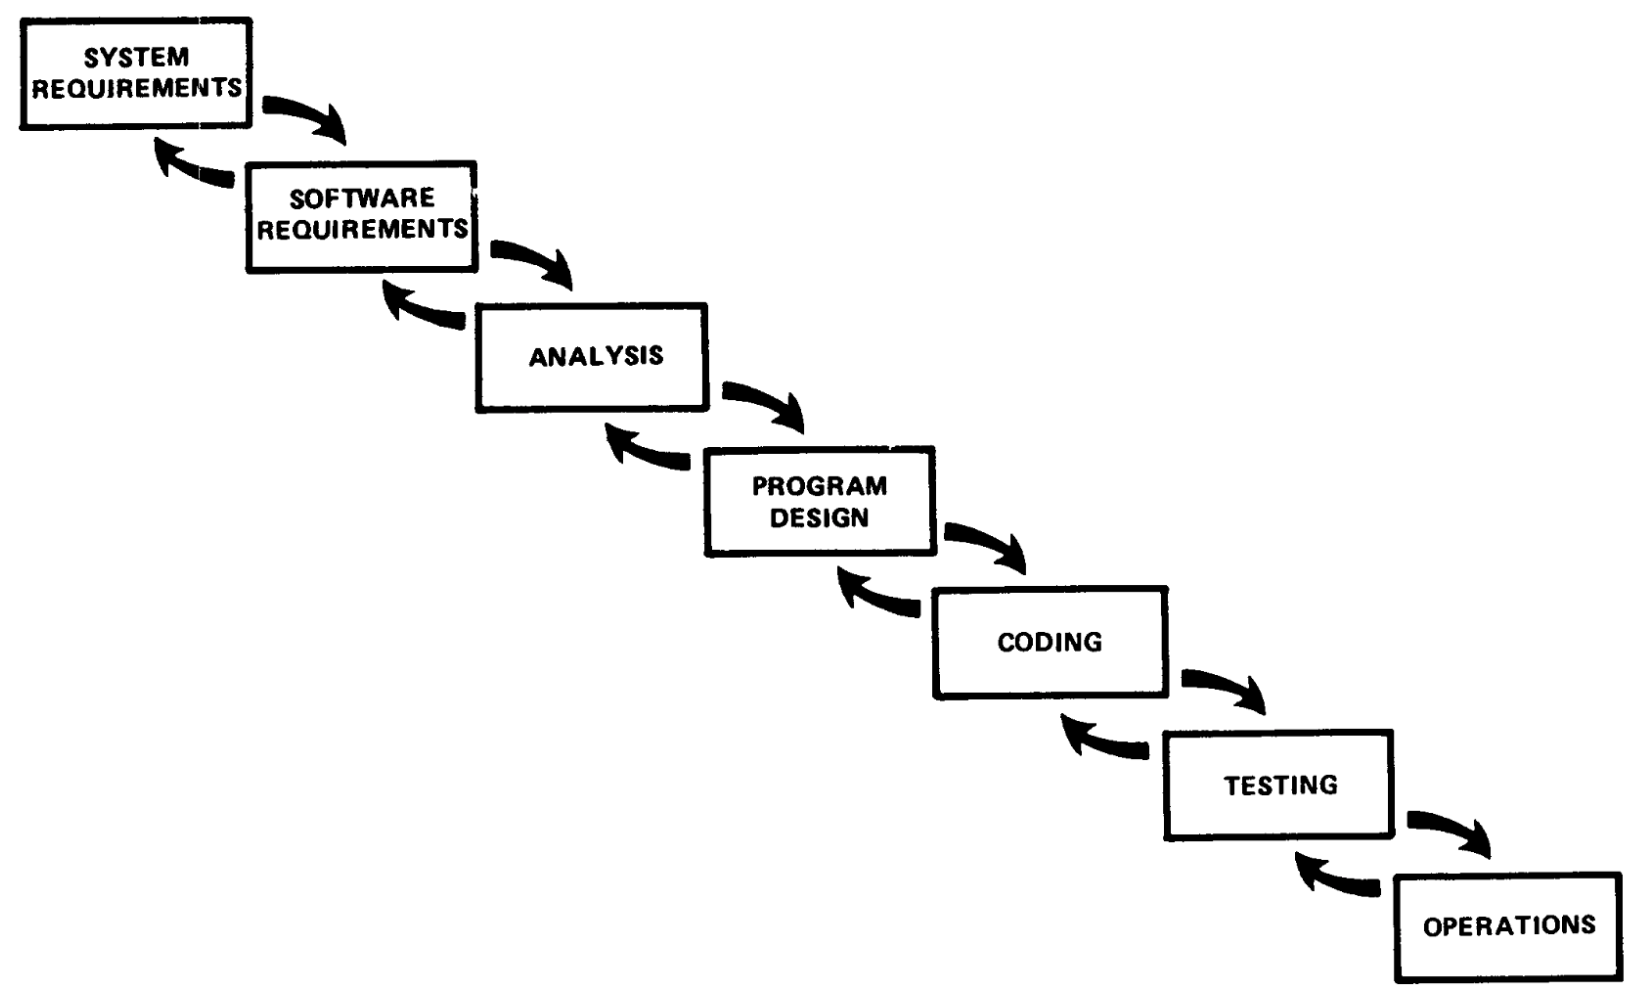
\includegraphics[width=0.9\linewidth]{img/royce-largePrograms}
	\caption{Vorgehensmodell nach Royce}
	\label{img:royce-largePrograms}
\end{figure}


Unsere Bedürfnisse deckt das Vorgehensmodell von Royce ~\cite{Royce1970}, welches in Abbildung  \ref{img:royce-largePrograms} dargestellt ist, am besten ab. Es besteht grundsätzlich aus einem sequentiellen Ablauf der Entwicklungsphasen, berücksichtigt dabei aber auch die Notwendigkeit von Rücksprüngen zur vorherigen Phase.
Die ersten Phasen von der Definition der "System Requirement" bis zu den ersten Gedanken zum Thema "Program Design" behandeln wir im Fachmodul. Der zweite Teil mit der genauen Definition des Programm Designs bis zum Betrieb der Software findet anschliessend während der Bachelor-Arbeitszeit statt.

\section{Entwicklungsprozess}

Den Entwicklungsprozess führen wir mit Kanban. Kanban basiert auf dem Pull-Prinzip d.h. jeder, der im Projekt arbeitet, holt sich selbst einen neuen Arbeitsauftrag, sobald er mit einem fertig ist. Die führt dazu, dass die Arbeiten speditiver abgewickelt werden und spart zudem die Stelle des Projektmanagers, der die Aufgaben verteilt.

\Diskussionspunkt{Bild Kanban-Board}

David Anderson \cite{AndersonDavidJ2011K:eC} hat das System Kanban, welches ursprünglich aus der Industrie kommt, auf die IT angepasst und dadurch das "Virtuelle Kanban System" entwickelt. Die grundlegenden Regeln daraus lauten:

\begin{itemize}  
\item Jede Karte ist eine Aufgabe
\item Die Aufgabe soll maximal 8-16h benötigen
\item Pro Spalte sind die Anzahl Karten limitiert
\item Eine neue Karte darf erst gezogen werden, wenn die vorherige fertig ist (Multitasking-Vermeidung)
\end{itemize}



\section{Projektplan für die Bachelor-Arbeit}
Hier wäre ein A3-Blatt quer noch cool. Darauf sollten alle Wochen von Start BA bis zur Abgabe sein.
Alle offiziellen Termine, alle Meilensteine usw.
Eine Zeile für Meetings (Führungsrhythmus)
Abhängigkeit der einzelnen Artefakte voneinander (evtl. mit MS-Project arbeiten)
Was gehört alles in eine Projektplan. Was ist der Unterschied zwischen Projekt- und Terminplan?

\section{Risikoanalyse}
\subsection{Risikoliste}
Ausgearbeitet mit dem Risikolexikon aus dem Buch xxxx, Risikoschablone
siehe ~\cite{AhrendtsFabian2008Il:w}.


\subsection{Risikoanalyse und Risikomatrix}





   
\Diskussionspunkt{Risikotabelle mit Wahrscheinlichkeit und Auswirkung gewichtet, Risikomatrix als Übersicht, Themen sind technische Umsetzung, Zusammenarbeit mit Dritten, Termine, Ressourcen, }



\section{Dokumentation}
\Diskussionspunkt{Versionsverwaltung, Dokumentationskonzept, Tools?, Printscreens}

%Allgemein
Für die Bachelor-Arbeit verwenden wir unterschiedliche Dokumentationswerkzeuge. Bei der Auswahl haben wir darauf geachtet, das die Tools kostenlos nutzbar und für sämtliche Plattformen verfügbar sind (Windows, Mac, iPad, usw.) Weiter war uns wichtig, dass die Tools untereinander kommunizieren können. 

% github / Trello / Toggl
Sämtliche Artefakte speichern wir auf \textit{github}. Wir haben somit eine automatische Versionierung der Dokumente und können unabhängig voneinander an den Dokumenten arbeiten. Die Planung bzw. Darstellung des Entwicklungsprozesses erledigen wir mir \textit{Trello}. Es ist ein intuitives Tool, welche diverse Integrationsmöglichkeiten mit den anderen Tools bietet. Für die Zeiterfassung verwenden wir \textit{Toggl}, welches mittels Plugin direkt in Trello integriert werden kann.

% Kommunikation nach aussen
Damit wir keine Besprechungsprotokolle verschicken müssen und dass alle Informationen für alle immer zugänglich sind, haben wir entschieden das Reporting in Form einer öffentlichen Webseite zu erstellen. github bietet mit \textit{GitPages} einen Hosting-Service an, der genau dies ermöglicht. Der Vorteil von GitPages ist, dass wir sämtliche Daten in einem einzigen Ort bzw. Repository vereint haben. Damit wir uns nicht mit Formatierung u.a. herumschlagen müssen und uns auf den Inhalt konzentrieren können, verwenden wir \textit{mkdocs} als Template Engine. Die Webseiten-Einträge können wir dadurch auf simple Art in Form von Markdown-Files erstellen.

% Kommunikation nach innen
Innerhalb des Teams nutzen wir das Kommunikationstool \textit{Slack}. Dieses ermöglich uns Konversationen als Chat aufzuzeichnen und nach Themen zu gruppieren. Weiter lassen sich Dokumente austauschen. Sämtliche git-Posts werden von Slack automatisch geloggt und können, falls gewünscht, als push-Notification angezeigt werden.
Das wöchentliche Team-Meeting findet über \textit{Skype} statt, da wir den regelmässigen mündlichen Austausch aus zentralen Punkt erachten.

% Bericht = LaTeX
Den Bericht werden wir in LaTeX verfassen. Wir haben uns für LaTeX entschieden, da wir uns auf den Inhalt konzentrieren können und das Layout automatisiert ist. Weiter ist LaTeX in der Wissenschaft weit verbreitet. Die Bachelor-Arbeit ist deshalb eine gute Gelegenheit uns in dieses Thema einzuarbeiten.


\section{Rechtliche Ansprüche}
siehe separates Dokument


%%%%%%%%%%%%%%%%%%%%%%%%%%%%%%%%%%%
%%  Schluss
%%%%%%%%%%%%%%%%%%%%%%%%%%%%%%%%%%%
\chapter{Schluss}
\Diskussionspunkt{Erkenntnisse, Einschätzungen}




%%%%%%%%%%%%%%%%%%%%%%%%%%%%%%%%%%%
%  Verzeichnisse
%%%%%%%%%%%%%%%%%%%%%%%%%%%%%%%%%%%
\bibliography{literatur}{}	
\bibliographystyle{plain}

\end{document}
